\documentclass[10pt,a4paper,oneside]{report}
\usepackage[utf8]{inputenc}
%Algemene documentinstellingen als dubbelzijdig, codering, rapportsoort etc.

\usepackage[dutch]{babel}
\usepackage[backend=biber,style=apa,sorting=nty,natbib]{biblatex}
\addbibresource{bibliografie.bib}
\DeclareLanguageMapping{dutch}{dutch-apa}
%APA-richtlijnen en taalinstellingen

\usepackage{afterpage}
\newcommand\blankpage{
    \null
    \thispagestyle{empty}
    \newpage}
%Code om blanke pagina's in te voegen
%Code is \afterpage{\blankpage}

\usepackage{graphicx}
\graphicspath{ {./Images/} }
%Om figuren in te voegen

\usepackage{fancyhdr} %Voet- en kopteksten
\usepackage{csquotes} %Quotes die Babel respecteren
\usepackage{lastpage} %Variabele voor paginanummering
\usepackage{booktabs} %Tabeloptimalisatie
\usepackage{pdfpages} %Samenvoegen van PDF's 
\usepackage{lipsum} %Lorem ipsum
\usepackage{color} %Tekstkleur
\usepackage{microtype} %Tegen de underfull errors en om justifying te helpen
\usepackage[pages=some]{background} %Achtergrondafbeeldingen bij voorwoord
\usepackage{comment}

\usepackage[linktoc=all]{hyperref}
\hypersetup{
    colorlinks=true,
    linkcolor=black,
    filecolor=cyan,
    urlcolor=cyan,
    citecolor=black,
    breaklinks=true,
    bookmarksopen=true}
%Links naar websites, bronnen, inhoudsopgave, pagina's etc.

\def\titel{Afstudeerwerkplan Seafood Connection}
\def\ondertitel{Convergerende uitwerking van de opdrachtformulering en -omgeving als hulpmiddel \\
voor de afstudeeropdracht bij Seafood Connection B.V. te Urk}
\def\auteur{Gerrit Post}
\def\studentklas{S1071236 --- AC4V}
\def\mailstudent{S1071236@student.windesheim.nl}
\def\telstudent{+31 642 678 172}
\def\school{Hogeschool Windesheim}
\def\domein{Accountancy, BMR}
\def\mailschool{a.vanden.brandhof@windesheim.nl}
\def\organisatie{Seafood Connection B.V.}
\def\mailorganisatie{info@seafoodconnection.nl}
\def\telorganisatie{+31 527 687 066}
\def\docent{Drs. A. Dannenberg RA}
\def\begeleidereen{L. Brouwer, MSc.}
\def\begeleidertwee{J.J. Molenaar, MSc.}
\def\datum{21 september 2018} %Alle variabelen in het document als titel, datum etc.

\title{\titel}
\author{\auteur}
\date{\datum}
%Documenteigenschappen worden hier gekopieerd uit Definities.tex

%EIND VAN PREAMBLE


\begin{document}
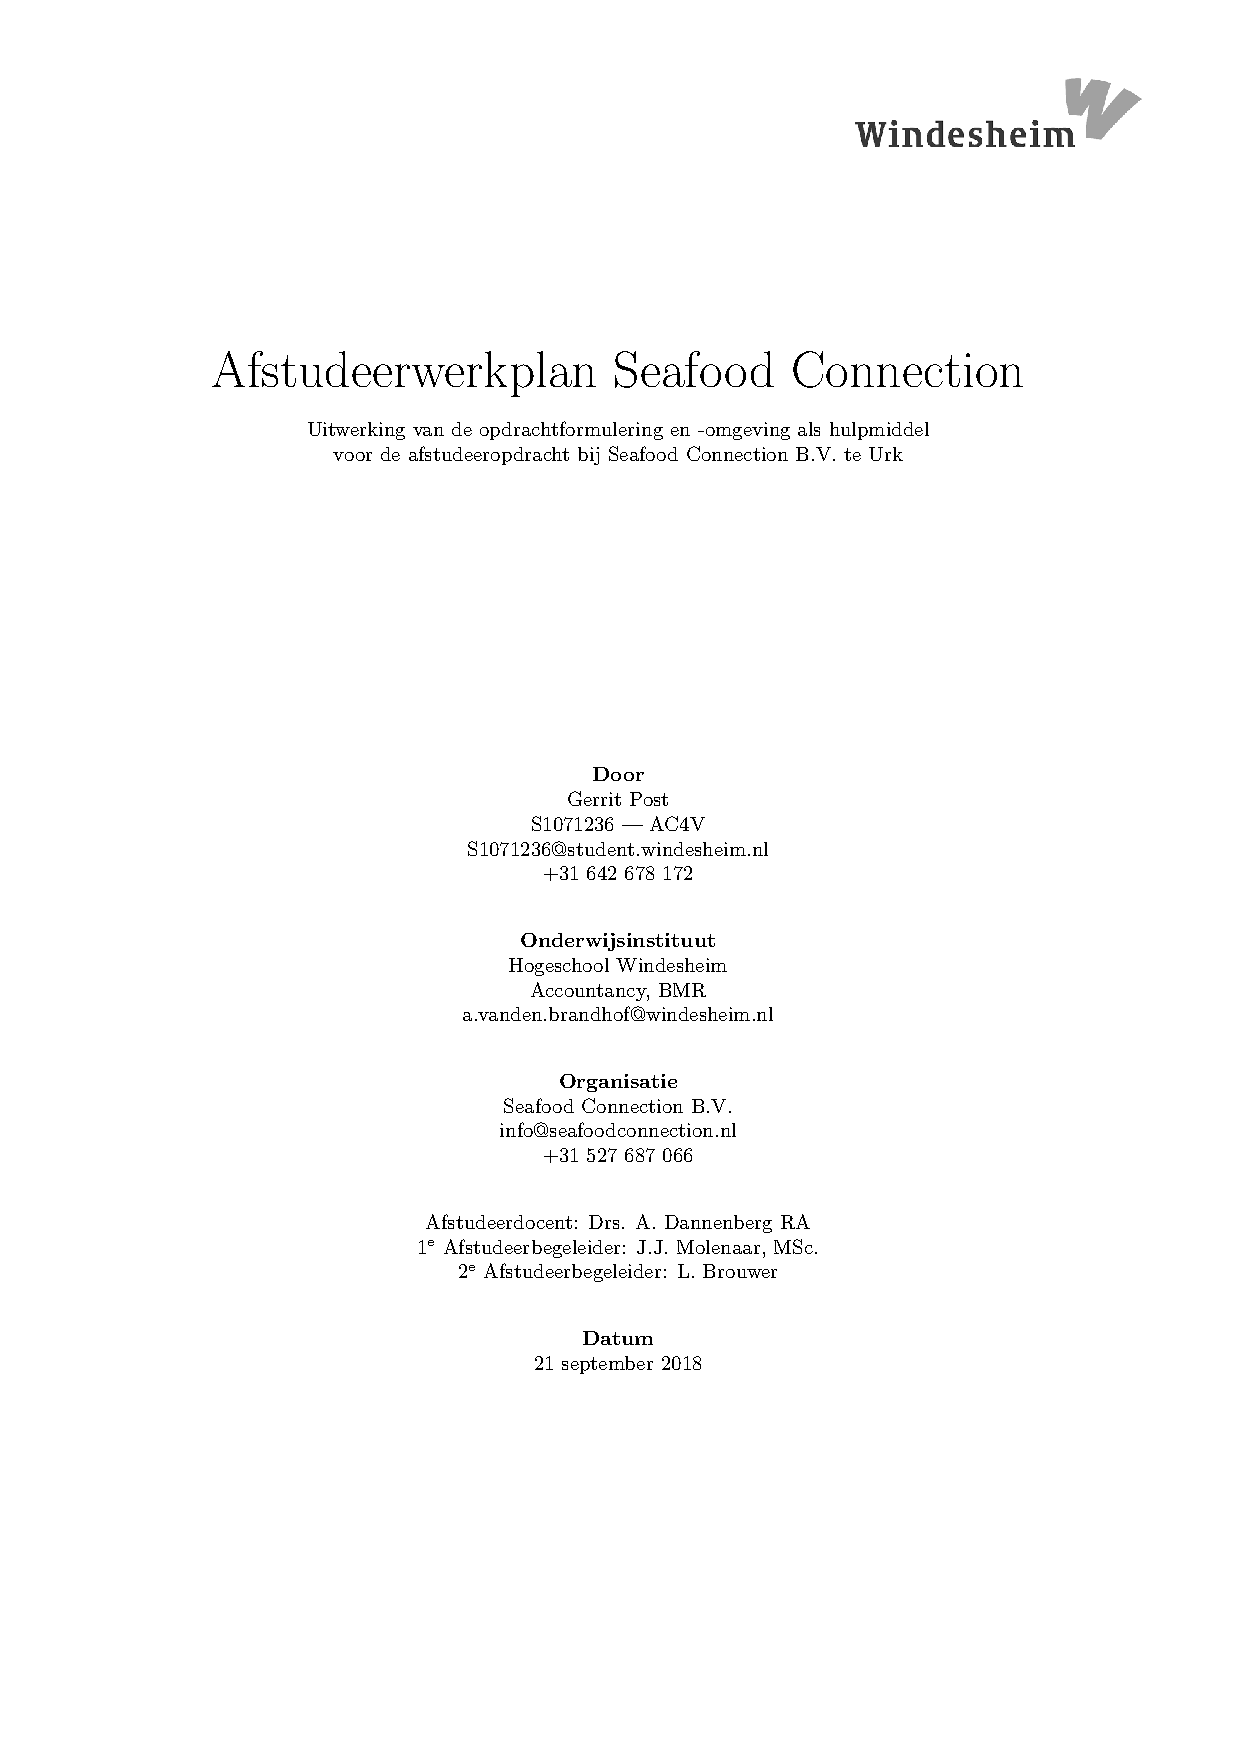
\includepdf{./Titelpagina/titelpagina.pdf}
\afterpage{\blankpage}
\backgroundsetup{contents=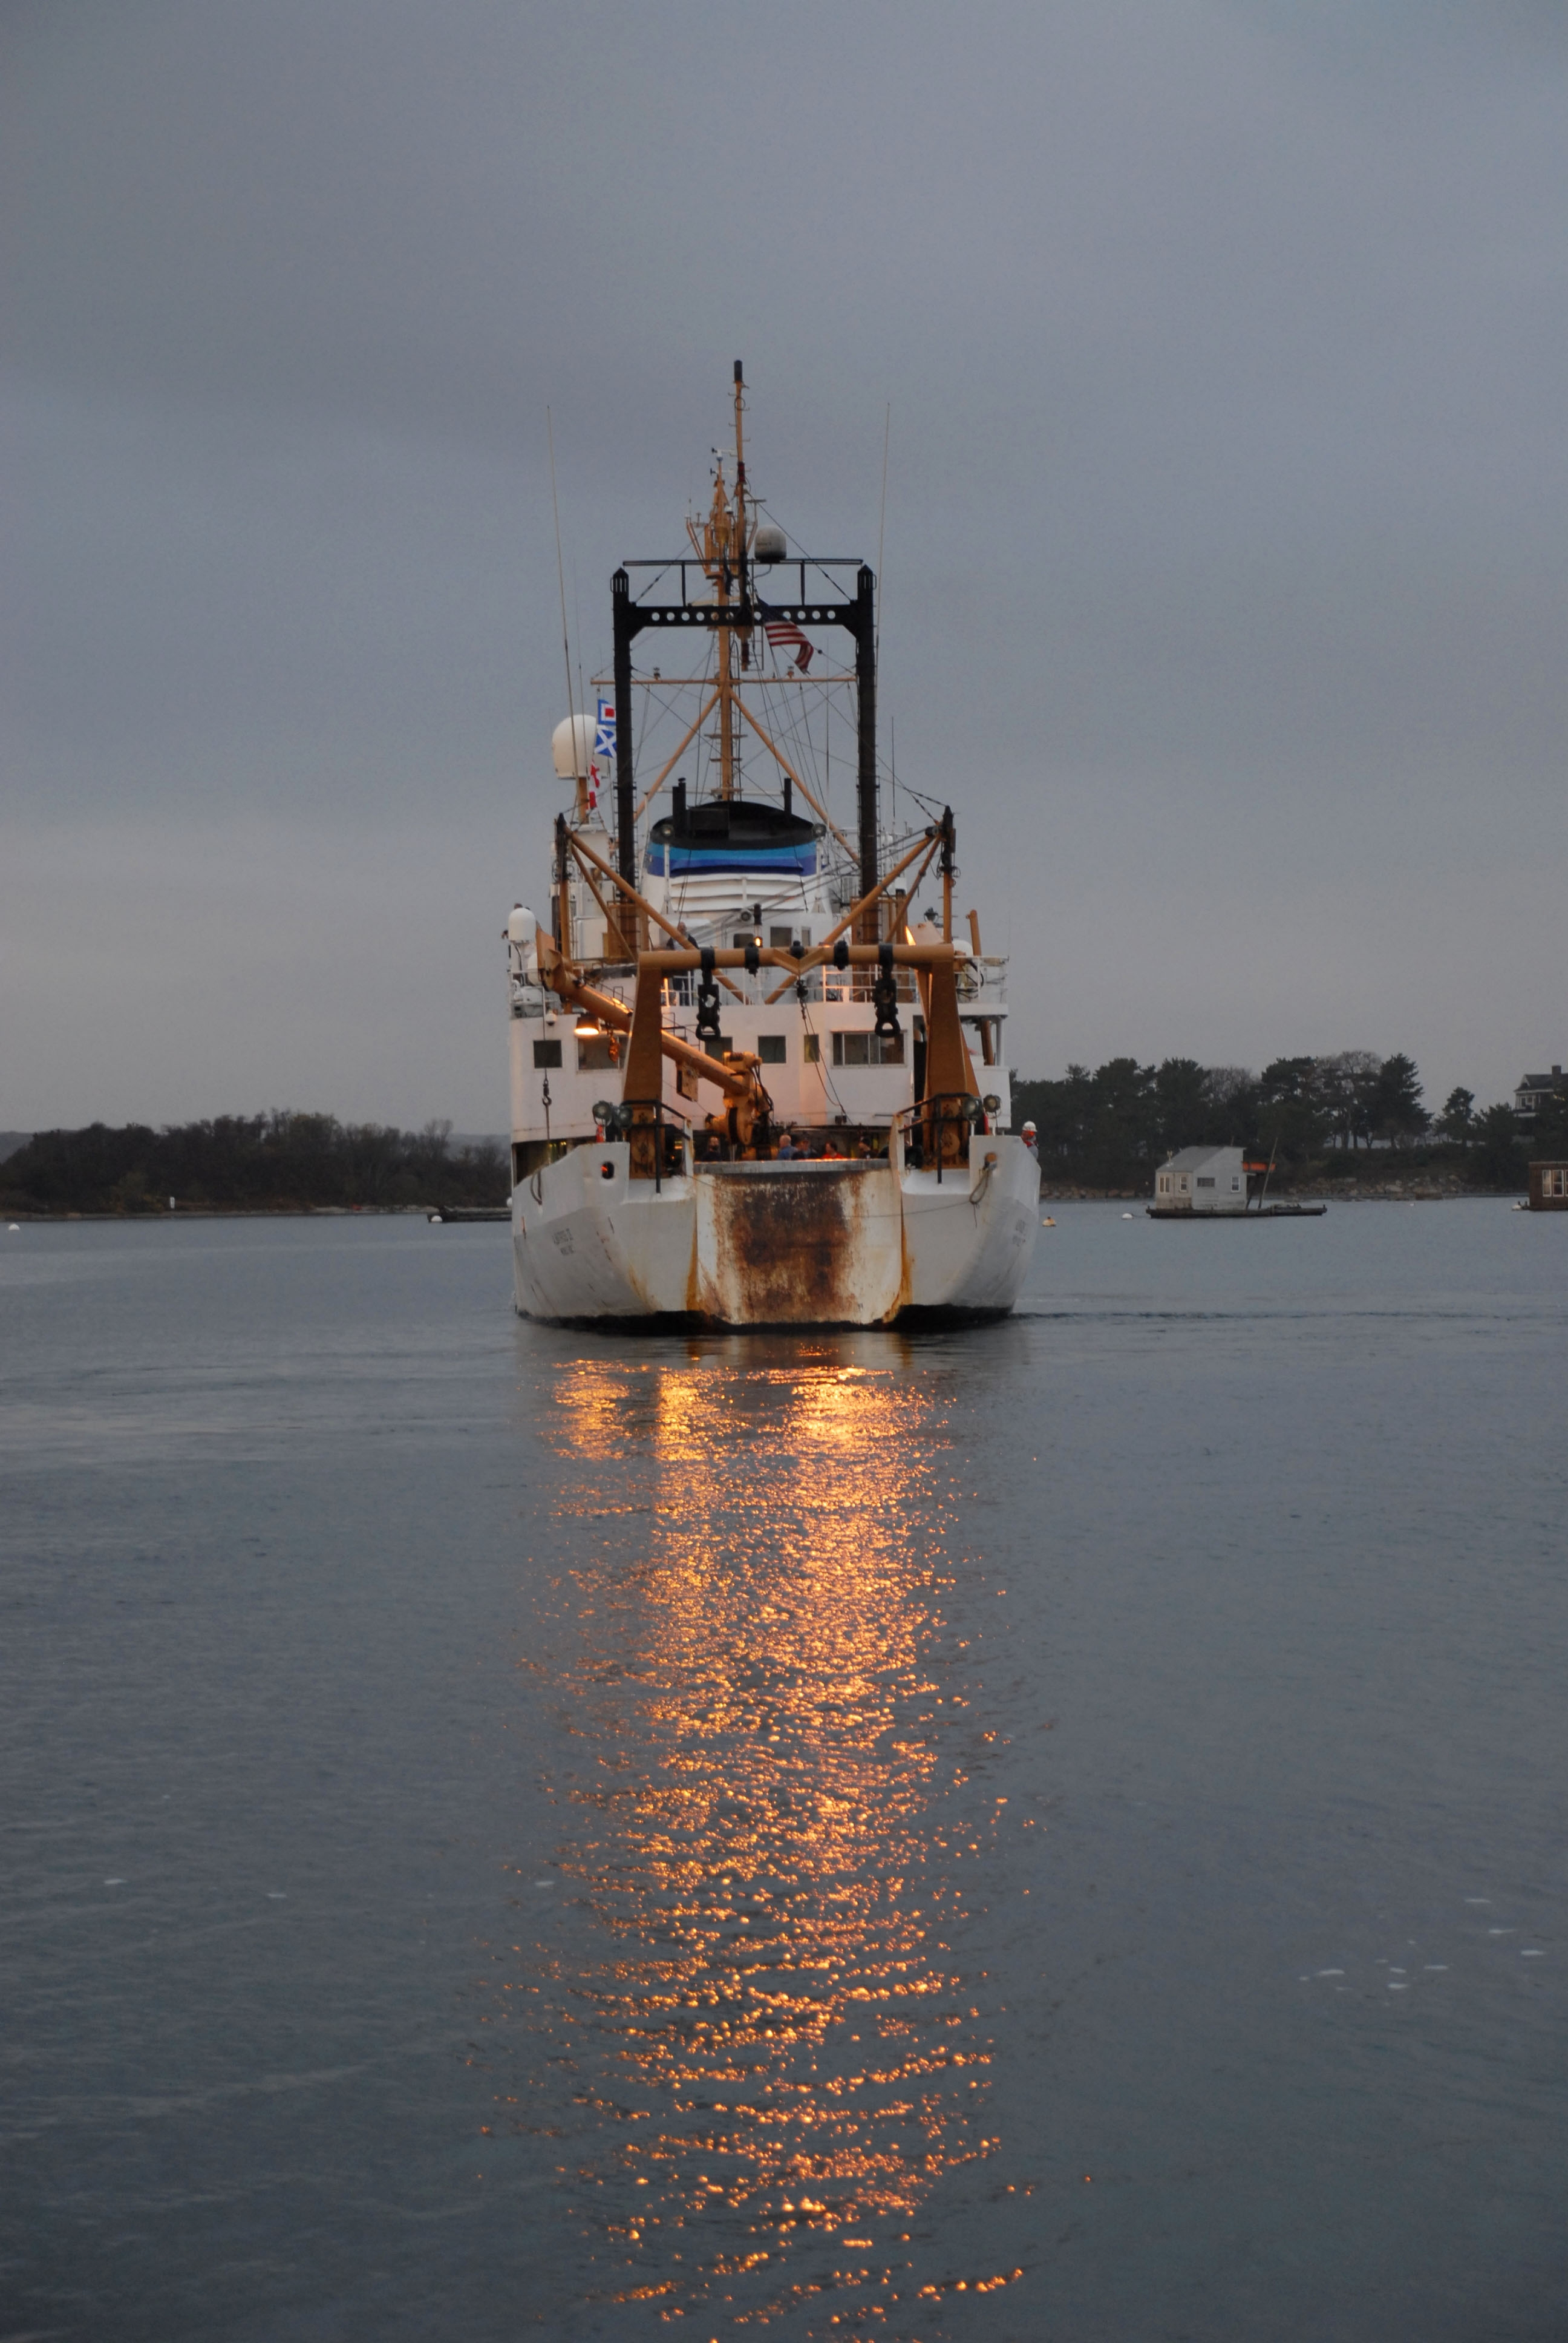
\includegraphics{3},angle=0,scale=1,opacity=1}
\BgThispage
%Titelblad wordt geïmporteerd als PDF want die is oneside en dit document twoside, zie eerste regel
%Na titelblad een lege pagina zodat er niets op de achterkant staat als hij dubbelzijdig wordt geprint

\chapter*{Voorwoord}
\thispagestyle{empty}
\backgroundsetup{contents=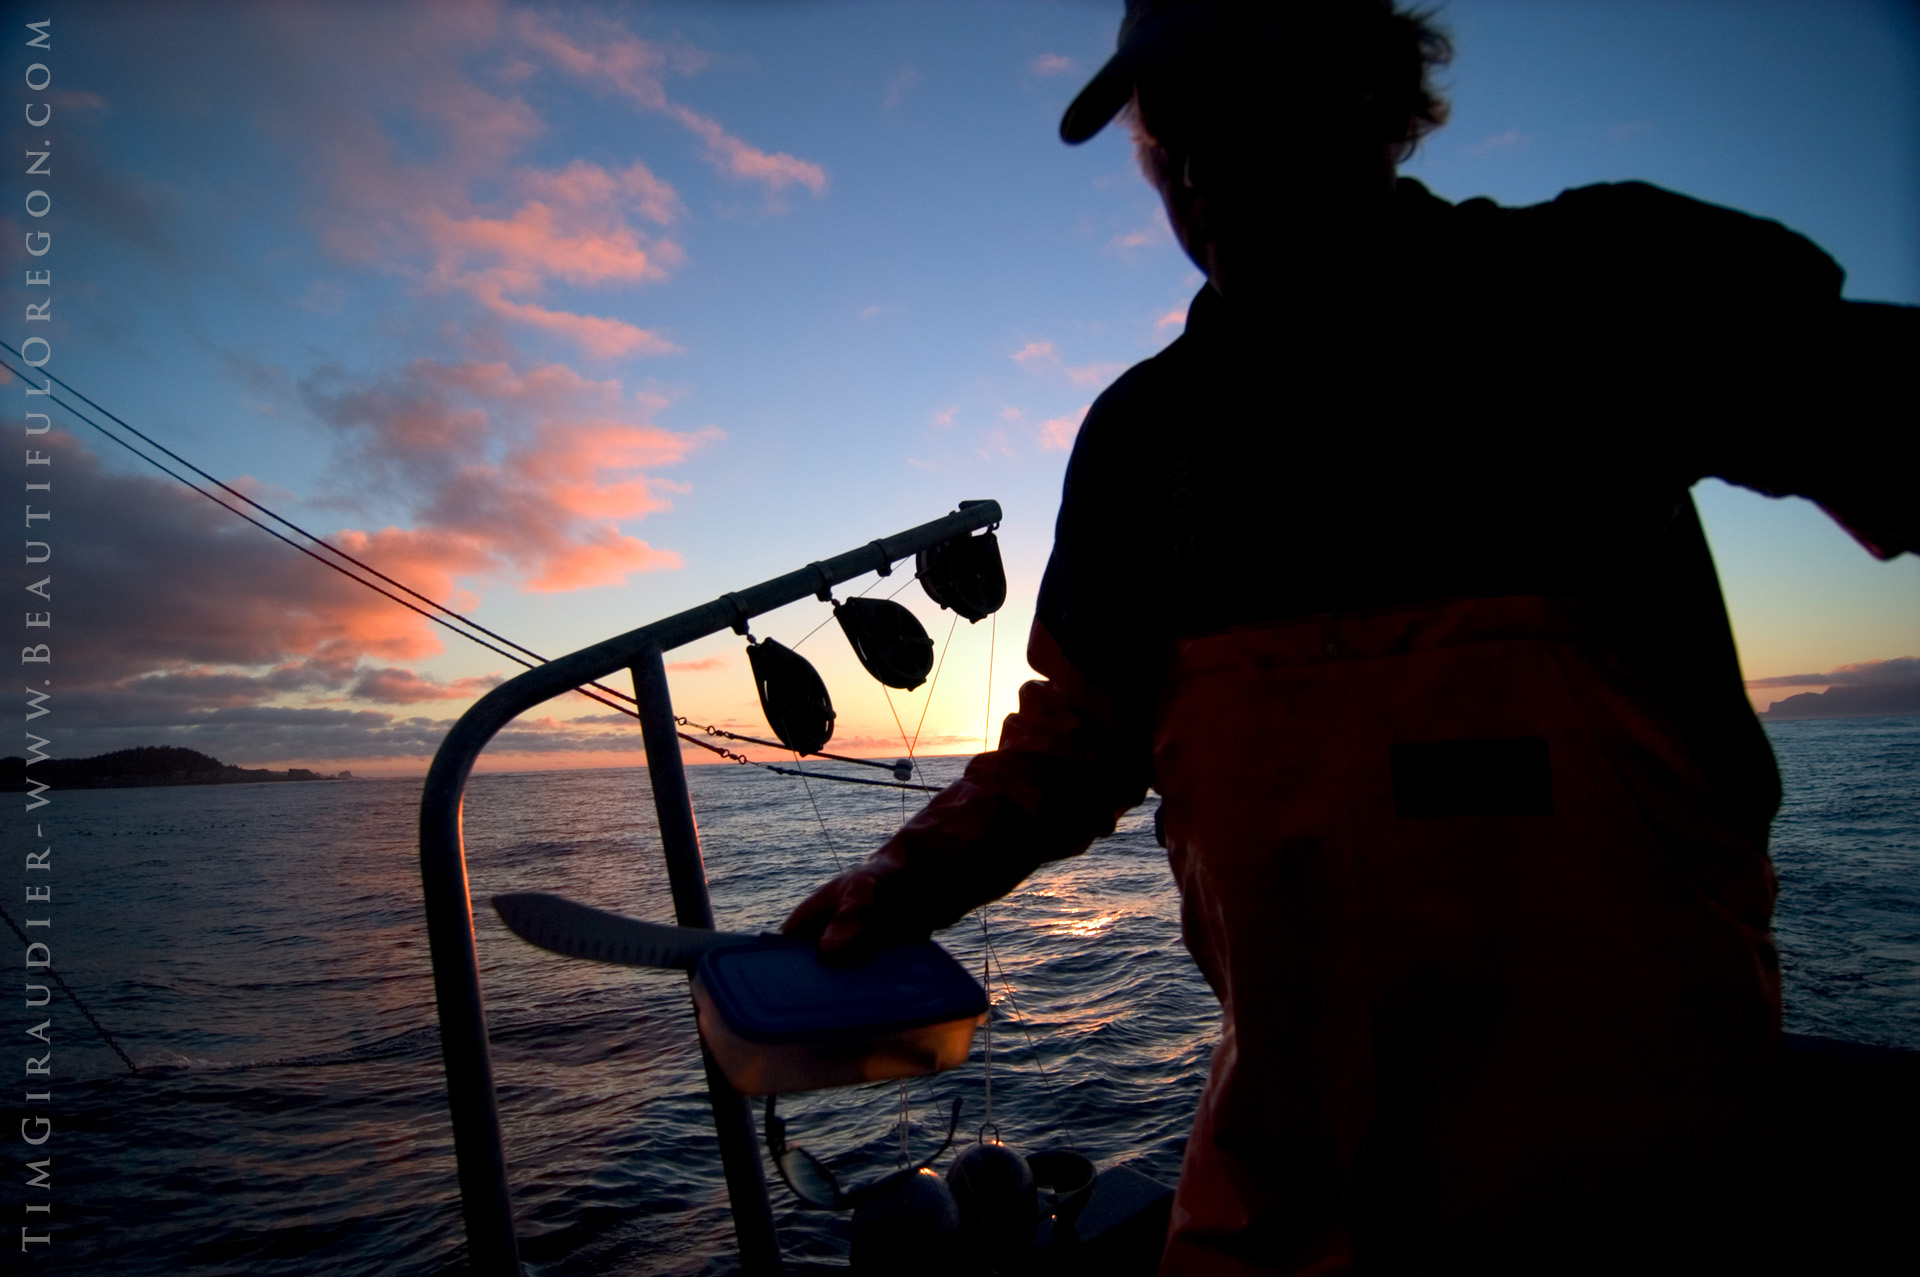
\includegraphics{7},angle=-2.5,scale=0.68,opacity=0.60,hshift=150}
\BgThispage
Het maken van een afstudeerproduct is een logische en verplichte laatste stap voor het afronden van mijn bacheloropleiding aan de Windesheim te Zwolle. Al voor de opdracht van start was gegaan was ik zeer geïnteresseerd om deze afstudeerstage uit te kunnen voeren bij een uitdagende en atypische opdrachtgever. Dit verlangen was vooral gegrond in het feit dat ik een affiniteit voor AO/BIV aan het ontwikkelen was en graag wilde toetsen of mijn kennis op dit vakgebied voldoende is. En waar beter deze kennis te toetsen dan bij een werkgever waar niet zomaar de geleerde typologieën gekopieerd en geplakt kunnen worden?
Mijn zoektocht begon naar een organisatie die in dit profiel past en graag met mij samen zou willen werken aan een nuttig eindproduct.

Eind juni kwam ik op de tennisbaan in gesprek met oud-collega Jurian, hier kwam Seafood Connection ter sprake als een interessante organisatie voor mij als afstudeerder. Al snel zat ik aan tafel met CFO Lucas Brouwer en voorgenoemde Jurian Molenaar waar Seafood Connection een steeds interessantere kandidaat leek te worden. Ik ben blij met de samenwerking die wij zijn aangegaan en ik hoop op een vruchtbare en productieve afstudeerperiode. Een bijzondere dank aan Rienk Bouma, Jon Bergsma, en Alidus Dannenberg voor de begeleiding vanuit school bij het formulerende proces van de opdracht. 

Ik wens de lezer veel plezier bij het lezen van dit afstudeerwerkplan en vanzelfsprekend ben ik bereid om vragen te beantwoorden en mee te nemen voor de opdracht.

\bigskip
\noindent
\textbf{Gerrit Post} \\
\textit{Student Accountancy, Hogeschool Windesheim}

%\vfill
%{\footnotesize\textsf{\textcolor{white}{Giraudier, Tim (2018). Cross Sound, Alaska.}}}

%Voorwoord met achtergrondafbeelding

%\chapter*{Samenvatting}
%\thispagestyle{empty}
%\lipsum[1-4]

\setcounter{page}{3} %Door importeren van PDF klopt paginanummer niet, hierbij gecorrigeerd
\tableofcontents
\thispagestyle{empty}


\chapter*{Inleiding}
\addcontentsline{toc}{chapter}{Inleiding} %Ongenummerde chapters komen niet in de ToC, met deze code wel
Om duidelijk de uit te voeren opdracht te definiëren en te verkennen wordt in dit verslag met een brede blik gekeken de probleemformulering, -omgeving, en er wordt onderzocht wat er concreet gaat spelen bij dit onderzoek. In samenwerking met de finance afdeling van Seafood Connection (hierna als afkorting: SFC) wordt georiënteerd op de opdrachtformulering en wordt ook de opdrachtomgeving bekeken aan de hand van een uitgebreide bedrijfsverkenning. 

Om de lezer een goed beeld te geven van de opdrachtomgeving wordt eerst uitgebreid, maar doelgericht, de bedrijfsachtergrond beschreven. Vervolgens wordt de eerste stap van de onderzoekscyclus uitgewerkt volgens het model van Nel Verhoeven waar de probleemomschrijving breed en diep wordt uitgewerkt. In hoofdstuk drie wordt dit probleem omgezet in een concreet ontwerp waarin concreet wordt nagedacht over de invulling van de afstudeeropdracht- en periode. De competentieontwikkeling in hoofdstuk vier beschrijft de manier waarop de afstudeerstagiair gaat werken aan de competentie- en ontwikkelingspunten. Als slot vindt u de bronnenlijst, de bijlagen die verdiepend zijn voor dit plan, en de tijdsplanning voor de afstudeerperiode. 


\chapter{Bedrijfsachtergrond}
\section{De onderneming}
\subsection{Omschrijving}
Opgericht in 1995, door huidig CEO J. (Jan) Kaptijn en wijlen C. (Chris) Goos met het innovatieve idee om een geselecteerd assortiment visproducten aan te bieden over de hele wereld zonder zelf ook maar een enkele visverwerkingsband te moeten aanschaffen. Seafood Connection werkt nauw samen met landen over de hele wereld om lokaal visproducten aan te kunnen bieden met een hoge kwaliteitsstandaard. Deze standaard wordt gegarandeerd door contacten van het bedrijf zelf grondige controles uit te laten voeren bij de leveranciers op locatie. Daarnaast wordt het productie- en verwerkingsproces gehouden aan hoge Europese standaarden als IFS, BRC, MSC en HACCP. \citep{sfcwebsite}

In 2013 werd de meerderheid van Seafood Connection Holding gekocht door het Japanse Maruha Nichiro. Dit miljardenbedrijf, opgericht in 1880, is evenals SFC in alle uithoeken van de wereld te vinden. SFC hoopt met deze samenwerking te kunnen profiteren van de kennis en middelen van Maruha Nichiro, die naast de verkoop van visproducten het doel hebben om de hele waardeketen van de visindustrie te domineren. Dit betekent dat Maruha Nichiro een hand heeft in een groot aantal bedrijven dat rijkt van bedrijven in de aquacultuur, distributiecentrums en fabrieksschepen. Het moederbedrijf houdt het Nederlandse Seafood Connection nauwlettend in de gaten, dit doet zij door werknemers van Maruha Nichiro bij Seafood Connection op locatie te laten werken zodat zij periodieke rapportage kunnen versturen naar het hoofdkantoor in Japan. \citep{sfcwebsite,Visserijnieuws}

\subsection{Fase}
Seafood Connection opereert in een markt die deels gedefinieerd wordt door prijsconcurrentie, het leveren van visproducten met kwaliteitskeurmerken is niet een nieuw fenomeen. Het onderscheidend karakter moet vaak ergens anders vandaan komen dan het voldoen aan minimum kwaliteitseisen. 

Het onderscheidend karakter is bij SFC bij een aantal zaken te merken. Ten eerste is er door de jaren heen zoveel kapitaal verworven dat SFC in een bevoorrechte positie is waar zij op grote schaal kan inkopen. Tevens heeft SFC een select aantal leveranciers die nauwkeurig gekozen zijn op hun bereidbaarheid om vis te leveren die aan de normen SFC voldoen. SFC opereert in een verzadigde markt, maar groeit altoos door haar marktaandeel en het productaanbod.

\subsection{De activiteiten in perspectief} \label{beschr:activiteiten}
Om een volledig beeld te krijgen van de ondernemingsactiviteiten is het belangrijk om aandacht te besteden aan de financiële kant van de onderneming. Hier gebeurt namelijk iets opmerkelijks, wanneer bijvoorbeeld de financiële ratio's vergeleken worden met algemeen geaccepteerde normen scoort Seafood Connection, voor een handelsbedrijf, relatief slecht. Om deze ratio’s te beoordelen moeten zij eerst in context worden geplaatst, deze kunnen niet één-op-één vergeleken worden met normen die worden gehanteerd voor een regulier handelsbedrijf. Het is voor een bedrijf als SFC namelijk aantrekkelijk om relatief veel schulden op zich te nemen ten opzichte van haar bezittingen. SFC koopt grootschalig in voor verscheidene producten op een groot aantal markten. Dit betekent dat wanneer een grote hoeveelheid visproducten worden gekocht, het gebruikelijk is dat de levering doorgaans pas na één maand plaatsvindt. Na levering blijft de voorraad doorgaans twee maanden op voorraad voor het verkocht wordt, waarbij betaling van deze order één tot twee maanden na de aflevering van deze goederen plaatsvindt. In feite ontvangt Seafood Connection vaak pas na vier tot zes maanden na inkoop van het product pas haar geld terug. De ratio’s die hiermee verbonden zijn kunnen dus niet ontkoppeld worden aan de inherente eigenschappen van bulkinkoop op een internationale markt. \citep{jaarrapport2017}

\begin{table}[h]
    \centering
    \caption{Kengetallen jaarrekening over 2017 \citep{jaarrapport2017}}
    \begin{tabular}{l r r}
        \toprule
        \textbf{Kengetal} & \textbf{Ultimo 2017} & \textbf{Ultimo 2016} \\
        \midrule
        Rendament TV & 5,6\% & 4,9\% \\
        Solvabiliteit & 24,6\% & 20,8\% \\
        Liquiditeit & 0,55 & 0,53 \\
        \bottomrule
    \end{tabular}
    \label{tab:kengetallen}
\end{table}

Uit het jaarrapport over 2017 worden de financiële ratio’s uit tabel \ref{tab:kengetallen} ontleend. Deze cijfers gelden voor de peildatum van respectievelijk 31 december 2017 en 2016.

Het rendement op het totale vermogen is berekend als ((nettowinst + betaalde rente) / balanstotaal), de solvabiliteit als (eigen vermogen / totaal vermogen), en de liquiditeit als ((vlottende bezittingen + liquide middelen) / kortlopende schulden). \citep{jaarrapport2017}

\newpage
\section{De organisatie}
Het is belangrijk om te verkenning hoe de organisatie is opgebouwd, niet alleen omdat dit een opdracht is die kijkt naar de administratieve \textit{organisatie}, maar ook omdat de organisatie van Seafood Connection veranderd is sinds de laatste keer dat er kritisch is gekeken naar de AOIB. Sinds die tijd is er haast een verdubbeling geweest van het aantal medewerkers van Seafood Connection B.V., de omzet is verdubbeld, en de indeling van afdelingen is veranderd door deze opnieuw in te richten zodat zij onder andere beter kunnen focussen op deelmarkten, (nieuwe) producten, en geografische gebieden. Om dit alles overzichtelijk te maken voor de probleemomgeving wordt in dit hoofdstuk de organisatie van Seafood Connection B.V. uitgewerkt. 

\subsection{Typering}
Seafood Connection is een handelsbedrijf in diverse diepvries visproducten met daarnaast in beperkte mate doorstroom van eigen goederen met een eenvoudig, technisch omzettingsproces \citep{aoibsfc}. Voor de verschillende bedrijfsactiviteiten fungeert Seafood Connection als:

\begin{enumerate}
    \item Handelsbedrijf dat hoofdzakelijk aan andere bedrijven levert
    \item Productiebedrijf met homogene massaproductie
    \item In zeer beperkte mate dienstverlening aan derden (door commissie op verkopen aan derden)
\end{enumerate}

Volgens de modellen van Starreveld is SFC een \textit{Handelsbedrijf op rekening}. Belangrijke aanknopingspunten voor de interne controle zijn de geautoriseerde brutomarge en prijsprocedure; de harde functiescheiding tussen de afdelingen: inkoop, opslag, verkoop en administratie; én de inventarisatie als het sluitstuk van de geld-goederenbeweging. In de grotendeels zelf-gerapporteerde quick scan geeft SFC zelf aan dat procedures verankerd in het systeem liggen, maar tegelijkertijd flexibel zijn voor optimalisatie; er is een sterke functiescheiding tussen inkoop, opslag en administratie. Echter geeft zij zelf aan dat er sprake is van een open magazijn, dat niet in eigen beheer is, en door derden alleen beheerd wordt door de magazijnmeester, terwijl het magazijn door verschillende mensen wordt geïnventariseerd, en ook er is sóms onafhankelijke controle van de verkoopprijzen. \citep{bivperspectief,quickscan}

Een ander belangrijk detail voor de Administratieve Organisatie is dat het bedrijf in sterke mate gebruik maakt van automatisering. Zo is er een bevoegdheidsmatrix waarin beschikkende medewerkers geautoriseerd of geblokkeerd zijn om bepaalde handelingen uit te voeren. Hier valt de opmerking te plaatsen dat er voor het afschermen van valutarisico's geen limitieten zijn voor de hoeveelheid in te kopen valuta. Dit is opzettelijk gekozen zodat de inkopers snel kunnen handelen bij veranderende koersen en niet een bureaucratisch proces hoeven te doorlopen om grote bedragen in te kopen. In de quick scan geeft de organisatie weer dat (bijna) altijd gebruik wordt gemaakt van automatisering. \citep{quickscan}

\subsection{Inrichting}
Seafood Connection is vijftig gemotiveerde werknemers sterk. Het kantoor op Urk vervult alle bedrijfsfuncties grotendeels op één locatie; er zijn enkele medewerkers werkzaam bij een klein, lokaal productieproces, namelijk bij de zagerij van Coldstore Urk waar een groot deel van de voorraad van SFC zich bevindt. De organisatie heeft vier niveaus: het managementteam (MT) dat de strategie formuleert, de unitmanagers (UMO) die hun afdelingen aansturen, managers die het aanspreekpunt zijn voor hun deelprocessen in de verschillende afdelingen, én assistants die de afdelingen ondersteunen met verschillende werkzaamheden. SFC is een lijn-staforganisatie met een gedeelde P-, G-, en M-indeling opgedeeld in de afdelingen: inkoop, opslag, verkoop, finance, ICT and production, HRM, compliance, en marketing verdeeld over vier segmenten: wholesale, retail, industry, en group companies (geografisch beheer). \citep{quickscan}

\section{De branche}
Kenmerken voor succes in de branche zijn ogenschijnlijk het hebben van een affiniteit voor duurzaamheid, naleving van kwaliteitsstandaarden en goed toegankelijk zijn zodat visproducten in elk jaargetijde geleverd kunnen worden. In mindere mate is er ook sprake van prijsconcurrentie, omdat alle visverwerkers uit dezelfde vaargebieden de vis vangen. 

Seafood Connection is niet de enige aanbieder van vis. SFC opereert op Urk, één van de grootste centrums voor de visverwerking in Nederland, de CFO van Seafood Connection zegt hier zelf over dat het een gezonde hoeveelheid concurrentie voor de kiezen heeft. Het is dan ook niet verrassend dat de onderneming als grootste succescriteria heeft gekozen om te winnen in de markt, dit plaatst zij boven criteria als het beschikken over een zo uniek en nieuw mogelijk productassortiment of efficiënte bedrijfsvoering. 

De missie van Seafood Connection is om het volgende te anticiperen: klantbelangen, de behoefte aan duurzame visproducten, en nieuwe trends. De onderneming wil dit realiseren door nieuwe partners te verkrijgen in cruciale markten in Europa, Amerika en Azië. Tevens worden nieuwe keteninnovaties verkregen door fusies en overnames in de visindustrie. \citep{sfcwebsite}

\bigskip
\noindent
\color{red}
Indien relevant ook nog: Gevolgde strategie, concurrentie, marktfactoren, belangrijke regelgeving. Oordeel van de accountant
\color{black}

\chapter{Onderzoeksvoorstel}
\section{De aanleiding}
\subsection{Probleemomschrijving} \label{beschr:problemen}
De AOIB bij Seafood Connection is in lichte mate verouderd, concreet betekent dit dat sinds de laatste update er nieuwe afdelingen zijn ontstaan, er nieuwe functies zijn gecreëerd of zijn veranderd, en dat het organogram veranderd is. Het bedrijf is sinds de laatste update verdubbeld qua omzet en personeel. Een update is dus hoognodig om te voorkomen dat de vastgelegde AOIB niet overeenkomt met de werkelijkheid. Wanneer de vastgelegde AO niet overeenkomt met de werkelijkheid zal dit tot gevolg hebben dat er geen fundament is voor de interne beheersing van de bedrijfsvoering. \citep{bivpraktijk}

Juist door deze verouderde AO is er een verschil tussen de daadwerkelijke bedrijfsprocessen en de formele vastlegging hiervan. Het grootste knelpunt hier is de vastlegging van de organisatorische maatregelen rond de financiële geldstromen. Zoals eerder beschreven in paragraaf \ref{beschr:activiteiten} haalt Seafood Connection haar bestaansgrond uit het feit dat er op grote schaal wordt ingekocht en verkocht op een internationale markt. De geldgoederenstroom is een cruciaal deel van de bedrijfsvoering die op het moment niet uitgebreid en doordacht is vastgelegd. \citep{aoibsfc}

De organisatorische maatregelen rond de financiële geldstromen komen voort uit de AOIB, de aflegging van het beleid over financiële geldstromen is dus onlosmakelijk van de administratieve organisatie. Momenteel is er nog niet een vastgelegd document omtrent de \textit{treasury} dat aansluit op het beleid rondom geldzaken. Treasurybeleid is de manier waarop een onderneming haar \textit{treasures} (of ook: schatten) beheert. De praktische invulling van het treaurybeleid wordt omschreven in het door het management opgestelde treasury statuut. 
Dit statuut is \textbf{intern} gericht door in kaart te brengen hoe de verschillende processen rond de financiële beheersing horen te functioneren, er wordt bijvoorbeeld beschreven wie welke functie heeft in het geldgoederenproces en welke controles daarop uitgevoerd worden. \\
Ook is het statuut \textbf{extern} gericht aan stakeholders door de verantwoording die wordt afgelegd, door het management, over het geldbeheer. \citep{ede,handreiking}
\newpage \noindent
In deze en volgende rapportage wordt de volgende definitie gehanteerd voor de term treasury statuut: 

\begin{displayquote}
Het treasury statuut is een door het management opgesteld rapport waarin de bevoegdheden, verantwoordelijkheden, toezichtmaatregelen, de sturing, en beheersing geformuleerd worden ten aanzien van financiële vermogenswaarden, financiële geldstromen, financiële posities en de hieraan verbonden risico’s. \\
\citep{handreiking} \label{def:treasury}
\end{displayquote}
\noindent
Zie ook \hyperlink{bij:treasury}{bijlage 1} voor een overzichtelijke uitwerking van het begrip treasury statuut.

Samenvattend worden de huidige bestaande organisatorische maatregelen en processen in kaart gebracht. Daarnaast is het management van SFC bewust dat er op een navolgbare en verantwoordelijke manier omgegaan moet worden met financiële middelen; immers handelt het bedrijf met een uitputbare hoeveelheid vreemde valuta en is er een hoge mate van liquiditeit vereist om het bestaan van het bedrijf in de toekomst te kunnen garanderen. Het treasury statuut is onlosmakelijk verbonden met de AOIB, het is daarom noodzakelijkk dit product pas wordt opgesteld wanneer de AO weer aansluit op de werkelijkheid \citep{watisonderzoek,buunk,financiering}.

\subsection{Betrokken partijen}
Om de aanleiding duidelijk te krijgen is het belangrijk om in kaart te brengen wie precies de problemen hebben, welke rol zij spelen bij deze opdracht, en of er met deze partijen rekening moet worden gehouden. Hoofdzakelijk is het management de meest betrokken partij, omdat de opdracht vanuit de leiding ontstaan is en zij degene zijn die de AO nodig hebben om de onderneming te doen functioneren en te beheersen. \citep{bivperspectief}. De betrokken partijen bij dit probleem zijn echter niet alleen de leden van het management. De inrichting en het vormgeven van de organisatie heeft direct invloed op alle bedrijfsprocessen en de werknemers werkzaam in de waardeketen. Het is voor de beheersing van de processen belangrijk dat de afstudeerstagiair gesprekken aangaat met niet alleen de afdelingshoofden, maar ook de assistenten die direct onder leiding van het middenmanagement staan. Bij de dagelijkse werkzaamheden wordt niet bewust nagedacht over de administratieve maatregelen die voor SFC gelden, om deze reden is onderzoek noodzakelijk om onder andere te kijken of er in de praktijk bijvoorbeeld de navolging plaats vindt van de al dan niet aanwezige functiescheiding. Sturend in het onderzoek is het management die de informatieverstrekkers zijn en de uiteindelijke afnemer zullen zijn van het eindproduct. 

Een aantal partijen zijn \underline{niet} (volledig) betrokken bij het afstudeerproduct. Ten eerste is de primaire accountant van SFC niet deel van de belangendriehoek (de stagiair, de opdrachtgever, de opleidingsinstantie). Deze keuze is bewust door het management gemaakt omdat de AOIB intern gericht is en het treasury statuut een aflegging van de verantwoording is vanuit het management. Hoewel de accountant niet deel is van de belangendriehoek, zijn zij wel deel van de stakeholders. Elk jaar wordt door de accountant van de Seafood Connection groep een interimcontrole uitgevoerd. Bij deze controle wordt onder meer gekeken naar de rol van organisatorische inrichting en de kwaliteit van bedrijfsprocessen. \citep{jaarrapport2017}

Ook de deelnemingen, groepsmaatschappijen, joint ventures, en andere verbonden onderneming zijn niet deel van het onderzoek. Het productverslag is enkel de interne beheersing van Seafood Connection B.V.

\subsection{Ontstaan opdracht}
Deze opdracht is ontstaan vanuit de finance afdeling in het afgelopen jaar. Deze handelt registrerend en controlerend ten behoeve van de geldgoederenstroom. De intern beschikkende afdelingen –-- inkoop en verkoop --– werken nauw samen met finance voor de bewaking en afdekking van valuta- en koersrisico. Het management en de afdeling finance hebben samen een voorkeur voor een formeel vastgelegd beleid en zochten hiervoor een passende afstudeerder. Daarnaast was de licht verouderde AOIB toe aan vernieuwing.


\section{De doelstelling}
Zoals hiervoor beschreven wordt de bestaande AOIB bijgewerkt waarbij vervolgens een zogenaamde treasury statuut wordt opgesteld (zie paragraaf \ref{def:treasury}). Het statuut komt voort uit de AOIB. In dit treasury statuut legt het management verantwoording af over het kasmiddelenbeheer en dus ook over hoe valutarisico wordt bestreden. Deze aflegging van de verantwoording over de financiële middelen moet in lijn zijn met de getroffen, organisatorische maatregelen en de manier waarop het management idealistisch de geldstromen bewaakt en monitort. Het management geeft zelf aan dat het opstellen van dit statuut een hoognodig deel is van het onderzoek, aangezien er al een bestaande AO aanwezig is en dat het kasmanagement, hoewel grotendeels geautomatiseerd, nog niet formeel is vastgelegd. Bij de uitwerking van de update van de AO wordt door de organisatorische veranderingen (beschreven in paragraaf \ref{beschr:problemen}) ook rekening gehouden met nieuwe afdelingen, veranderde afdelingen, nieuwe organisatiestructuren, afdelingen die gericht zijn op nieuwe producten en nieuwe markten.

Bij deze ontwerpende opdracht is aan het einde van het afstudeertraject de AOIB bijgewerkt en in brede zin in kaart gebracht. Nadenken over de structuren en maatregelen, zoals dat in een AO-beschrijving gebeurt, is voor veel bedrijven belangrijk om niet alleen te kunnen groeien in de toekomst, maar ook om het bestaan van de onderneming enigszins te kunnen garanderen en om te toetsen of er niet ongeoorloofd middelen uit de onderneming wegvloeien.

Belangrijk om in gedachten te houden bij deze opdracht is dat deze opdracht zowel intern als extern is gericht. Intern wordt verslag gedaan over de administratieve organisatie en deze wordt geüpdatet. Het is dus niet de bedoeling dat derden dit document voor handen krijgen. Het op te stellen treasury statuut is echter wel bedoeld voor derden want het is een verantwoording van het management over hoe er wordt omgegaan met financiële middelen. Stakeholders kunnen met dit document helderheid krijgen op het valutabeheer van de onderneming. Bij de uitwerking van deze twee deelproducten moet de bedoelde doelgroep wel in het oog worden gehouden.

Om deze twee producten goed in kaart te brengen worden interviews en enquêtes gehouden met zowel unitmanagers (UMO’s) en assistenten. Het doel hiervan is om de werkelijk aanwezige AO in kaart te brengen. Bij de vraagstelling moet op een zo’n objectief mogelijke manier, en vanuit een theoretisch kader, gekeken worden hoe deze AO per afdeling is ingericht.


\section{De hoofdvraag}
\textbf{Uit welke aspecten is de bestaande Administratieve Organisatie en Interne Beheersing van Seafood Connection opgebouwd en waar zijn wijzigingen en/of aanvullingen wenselijk, mede in het kader van geldmiddelenbeheer voor financiële vermogenswaarden, geldstromen, en de hieraan verbonden risico's?}

\bigskip
\noindent
\color{red}
Uit welke aspecten is de bestaande Administratieve Organisatie en Interne Beheersing van Seafood Connection opgebouwd en waar zijn wijzigingen en/of aanvullingen wenselijk, mede in het kader van geldmiddelenbeheer?

\bigskip
\noindent
Hoe ziet de bestaande Administratieve Organisatie en Interne Beheersing van Seafood Connection er uit en waar zijn wijzigingen en/of aanvullingen wenselijk, en hoe kan deze AO gebruikt worden bij de verantwoording over het treasurymanagement?

\color{black}

\section{De deelvragen}
\begin{enumerate}
    \item Gezien de bedrijfsactiviteiten van Seafood Connection en de hierbij passende relevante typologie, welke organisatorische maatregelen en aanknopingspunten worden dan verwacht voor de interne beheersing?
    \item Hoe wordt de bestaande AOIB aangevuld gezien de verwachte maatregelen vanuit het theoretisch kader en de daadwerkelijk bestaande AO aan de hand van interviews en enquêtes?
    \item Hoe kan het management de bevoegdheden, verantwoordelijkheden, toezichtmaatregelen, de sturing, en beheersing formuleren ten aanzien van financiële vermogenswaarden, financiële geldstromen, financiële posities en de hieraan verbonden risico’s?
    \color{red} \item Stap van theorie naar praktijk. Onderwerp van deze deelvraag: treasury gebruiken om de diepte in te gaan met hedge accounting. 
    %Hoe kan de treasury statuut de kwaliteit van de financiële externe verslaggeving en administratie verbeteren? Hoe wordt het nu toegepast, welke verslaggevingsgrondslag? Is HA in overeenstemming met verslaggevingsregels?
    \color{black}
\end{enumerate}




\chapter{Onderzoeksontwerp}

%per deelvraag de randvoorwaarden (budget, tijdsplanning en toegankelijkheid bronnen e.d.) en de gekozen dataverzamelingsmethode(n), begipsafbakening

\begin{enumerate}
    \item Gezien de bedrijfsactiviteiten van Seafood Connection en de hierbij passende relevante typologie, welke organisatorische maatregelen en aanknopingspunten worden dan verwacht voor de interne beheersing?
    \begin{enumerate}
        \item Wat is de typologie van SFC? 
        \begin{itemize}
            \item Welke kenmerken typeren de organisatie?
            \item Speelt grootte van de organisatie een rol?
            \item Aanknopingspunten IC
        \end{itemize}
        \item Welke processen en afdelingen zijn aanwezig in de organisatie?
        \begin{itemize}
            \item Beschikkend, bewarend, uitvoerend, registrerend, controlerend ten op zichte van wat? Wie zijn de kernspelers in de geldgoederenbeweging?
            \item Welke afdelingen zijn gebruikelijk in de typologie? Welke functie en verantwoordelijkheden vervullen zij?
        \end{itemize}
        \item Welke relevante BIV/AO informatie is beschikbaar voor deze typologie?
        \item Hoe kan de vergaarde informatie gebruikt worden bij interviews en enquêtes?
        \begin{itemize}
            \item Wat is belangrijk om over na te denken / uit te werken?
            \item Zijn er onderwerpen onderbelicht in de bestaande AO die door het vergaren van informatie bijgevuld moet worden?
        \end{itemize}
    \end{enumerate}
\end{enumerate}



\begin{enumerate}
    \setcounter{enumi}{1}
    \item Hoe wordt de bestaande AOIB aangevuld gezien de verwachte maatregelen vanuit het theoretisch kader en de daadwerkelijk bestaande AO aan de hand van interviews en enquêtes?
    \begin{enumerate}
        \item Komen de beschreven functies en afdelingen in de bestaande AO overeen met het theoretisch kader?
        \begin{itemize}
            \item Noteer verschillen als speerpunten voor de vragen
            \item Hoe is het organogram sindsdien veranderd? Nieuwe afdelingen, functies of relaties?
        \end{itemize}
        \item Komt de bestaande AO/BIV overeen met de bestaande vastgelegde AOIB?
        \begin{itemize}
            \item Open vragen aan zowel assistenten als UMO's naar procesbeschrijving
            \item Vastleggen verantwoordelijkheden en machtigingen / rechten
        \end{itemize}
    \end{enumerate}
\end{enumerate}



\begin{enumerate}
    \setcounter{enumi}{2}
    \item Hoe kan het management de bevoegdheden, verantwoordelijkheden, toezichtmaatregelen, de sturing, en beheersing formuleren ten aanzien van financiële vermogenswaarden, financiële geldstromen, financiële posities en de hieraan verbonden risico’s?
    \begin{enumerate}
        \item Hoe worden de processen die te maken hebben met geldmiddelenbeheer ingericht in de geformuleerde AO?
        \item Waar kunnen risico's in het proces van geldmiddelenbeheer worden gevonden en hoe worden deze gemitigeerd?
    \end{enumerate}
\end{enumerate}






\begin{comment}

\section{Begripsafbakening}
Het derde onderdeel van de probleemanalyse omvat de begripsafbakening. Hierbij geef je duidelijk aan wat jij verstaat onder de begrippen die voorkomen in hoofd- en deelvragen. We noemen dit het operationaliseren van de begrippen.

\section{Theoretische ondersteuning}
\subsection{Het vakgebied}
Doordat deze opdracht feitelijk in twee delen is opgesplitst worden ook meerdere vakgebieden ontplooit bij de uitwerking van deze opdracht. De hoofdvraag zal voornamelijk AO-gericht zijn. Dit deel is bedoeld om de huidige administratieve organisatie / bestuurlijke informatieverzorging in kaart te brengen van Seafood Connection. Het tweede deel is in het kader van treasury management waar voornamelijk het vak financiering een rol gaat spelen, toch komen termen als hedge accounting vanuit de externe verslaggeving hier ook aan de orde.

\subsection{Theoriën en modellen}
Voor de uitwerking van de AO wordt voornamelijk de theorie van Starreveld gehanteerd waarin per organisatietypologie onder andere wordt uitgewerkt welke preventieve en repressieve maatregelen verwacht worden. Door dit model slim te benutten en verschillende typologieën te combineren zal het mogelijk worden om een theoretisch kader voor SFC te maken. 

Het COSO Internal Control Framework wordt nadien uitgewerkt om de organisatie als geheel te kunnen omschrijven. In deze internationale standaard komen de volgende organisatorische onderwerpen aan de orde:
\begin{itemize}
    \item Controleomgeving
    \item Risicoanalyse
    \item Controle activiteiten
    \item Informatie en communicatie (managementinformatie)
    \item Monitoring
\end{itemize}
Ook wordt er gebruik gemaakt van het Portermodel en het 7S-model waarmee een externe en interne analyse van de onderneming wordt uitgevoerd.

\end{comment}













\chapter{Competentieontwikkeling}
\section{Persoonlijke ontwikkelpunten}
Ten behoeve van het persoonlijk functioneren en ontwikkelen voor de afronding van de bachelor opleiding accountancy, zijn de volgende ontwikkelpunten geformuleerd:
\begin{enumerate}
    \item Er worden stappen gezet om de communicatieve vaardigheden in woord en geschrift te versterken door voor interviews (met zowel de opdrachtgever als andere betrokkenen) goed na te denken over welke informatie benodigd is en hoe deze op een zo'n neutraal mogelijke wijze kan worden geformuleerd. Taalgebruik in rapportage wordt verbeterd door meerdere reviewers te vragen kritisch te kijken naar de rapportage en te doorgronden welke fouten worden gemaakt om verdere fouten te voorkomen. 
    \item Er wordt volgens een vast tijdsplan gestudeerd en gewerkt er een dwangmatige urgentie is om door te blijven werken. Dit wordt gerealiseerd door vaste routines op te bouwen en periodieke mijlpalen te stellen. Periodieke reflectie op de mijlpalen is hier ook belangrijk.
    \item Er wordt beter nagedacht over de toegevoegde waarde richting een potentiële werkgever en deze wordt op een eenduidige wijze geformuleerd. Dit wordt bereikt door te werken aan zo veel mogelijk werkzaamheden die relevant zijn met de accountancy opleiding als achtergrond. Concreet moet worden geformuleerd wat welke waarde kan worden toegevoegd die een andere afgestudeerde AC-student niet zou kunnen bieden.
\end{enumerate}

\newpage
\section{Landelijke beroepscompetenties}
Op de Windesheim community zijn een aantal onderzoekscompetenties geformuleerd om de afstudeerstudent te helpen bij het succesvol afronden van de scriptie. Een aantal hier van hebben betrekking op dit afstudeerwerkplan. Hier wordt verder toegelicht hoe deze competenties aan de orde zijn gekomen bij het opstellen van het AWP. \\
De afgestudeerde bachelor AC-student is in staat om: 
\begin{enumerate}
    \item Een probleemstelling te formuleren
    \item Voor de oplossing van het probleem beschikbare kennis te identificeren
    \item De kwaliteit van de kennis en de theorie die hem ter beschikking staat kritisch te beoordelen
    \item De basis van zijn analyse te modelleren
\end{enumerate}

\noindent
\textit{Ad. 1.} Er is hard en lang over de probleemstelling en aanleiding gediscussieerd met de opdrachtgever en gedeeltelijk met begeleidende docenten. De aanleiding was in de eerste fase van de opdrachtsformulering niet helemaal helder en er moest geschaafd en bijgesteld worden om een goede aanleiding en probleemomschrijving te formuleren. Het lijkt aan de ene hand tegenstrijdig, omdat wel meteen duidelijk was wat de doelstelling was en welke producten opgeleverd moeten worden. Juist door zo hard te denken over de probleemstelling in samenwerking met de betrokken partijen, is de huidige probleemstelling zo hard en onderbouwd. 

\bigskip
\noindent
\textit{Ad 2.} Alvorens het afstudeerwerkplan is opgesteld is er diep en breed gezocht naar enigszins relevante informatie uit een groot aantal soorten bronnen. Andere scripties, toegewijde vakliteratuur, en handreikingen vanuit het opleidingsinstituut waren hier het meest behulpzaam. De term \textit{treasury} (zie paragraaf \ref{def:treasury}) was voor deze verkenning niet compleet duidelijk. Er is voor dit onderzoek veel ingelezen over geldmiddelenbeheer om toch een voldoende geïnformeerde uiteenzetting te geven in de probleemomschrijving. 

\bigskip
\noindent
\textit{Ad. 3.} Er is, met afstemming met de opdrachtgever, een realistisch te behalen eindproduct voor ogen gesteld. De afkadering en de van de grenzen die zijn gesteld zijn bij beide partijen duidelijk en geaccepteerd.

\bigskip
\noindent
\textit{Ad. 4.} Het proces van het formuleren van de hoofdvraag en passende deelvragen was heel tijdrovend en was onderhevig aan veel veranderingen. Het uitwerken van meerdere mindmaps en causale veldmodellen hielpen hier enorm bij. Het zien van onderlinge verbanden was opbouwend en hielp om helder te zien hoe de opdracht opgedeeld zou moeten worden en welke informatie en deelstappen daarvoor nodig zouden moeten zijn.

\bigskip
\noindent
\color{red} Bron community ac \color{black}

\chapter{Tijdsplanning en communicatie}
Om er voor te zorgen dat er consistent gewerkt wordt aan het productverslag wordt er zo veel mogelijk gehouden aan de planning en normen die de school stelt en voorschrijft. Er wordt middels een eenvoudig Excel-bestand dagelijks bijgehouden hoe het aantal uren zich verhoudt ten opzichte van de opgelegde norm vanuit school. Er wordt een veiligheidsmarge van +10\% bijgeteld boven op deze urennorm. 

\begin{figure}[ht]
    \centering
    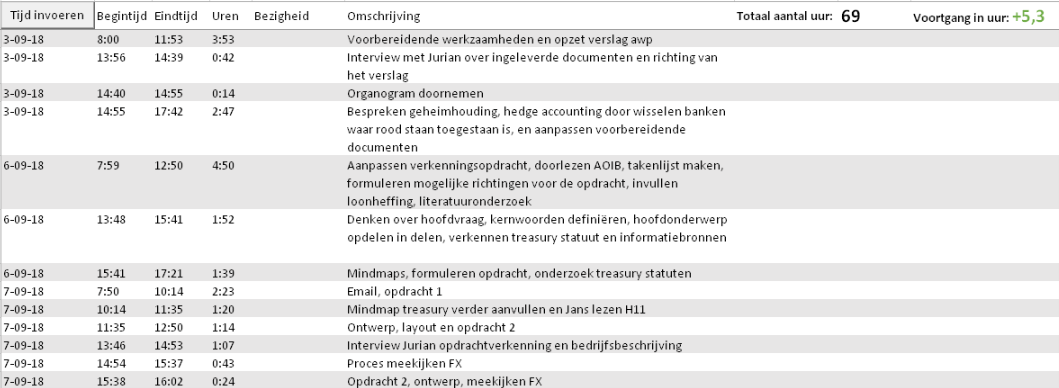
\includegraphics[angle=0,width=\textwidth]{tijdsplanning}
    \label{fig:tijdsplanning}
    \caption{Fragment van het dagelijks logboek met voortgang}
\end{figure}

Dit betekent ook dat er wordt gehouden aan de gestelde mijlpalen die voorgesteld worden in de afstudeerhandleiding. Deze planning is thuis en op de werkplek snel voorhanden zodat snel kan worden gezien of het tijdsschema op de lange termijn nog overeen komt.

\begin{figure}[ht]
    \centering
    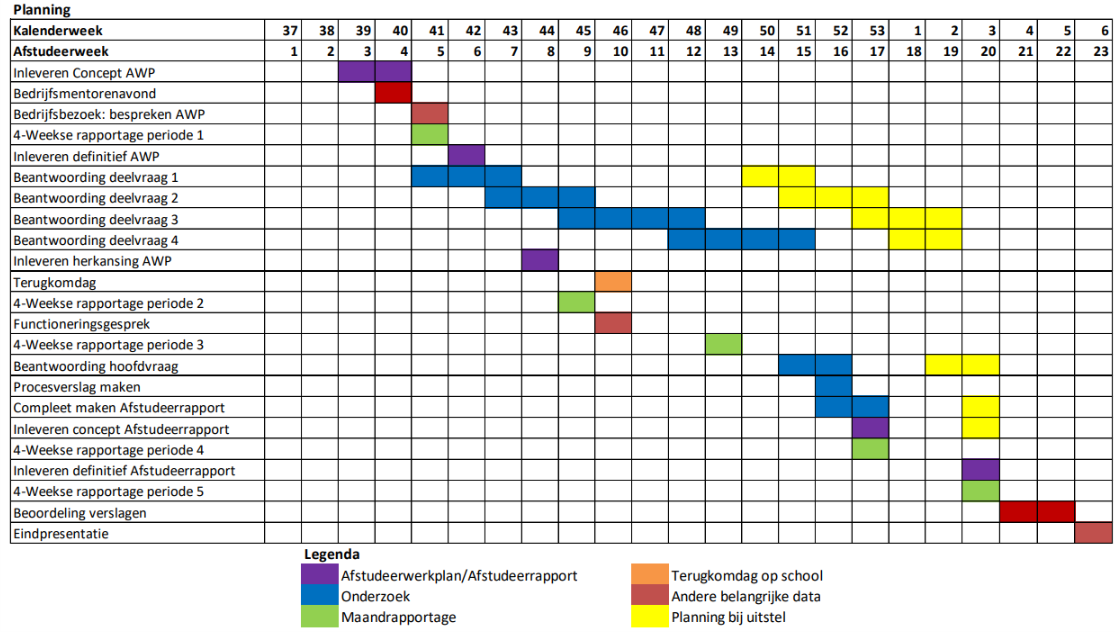
\includegraphics[angle=0,width=\textwidth]{planning}
    \label{fig:planning}
    \caption{Algemene planning afstuderen}
\end{figure}

Communicatie met de afstudeerdocent vindt plaats wanneer tijdens de uitwerking van het product- of procesverslag tegen problemen aan wordt gelopen waar teveel uren verloren gaan door het probleem zelf op te lossen of in overleg met de afstudeerbegeleiders. Het contact met de docent zal dus beperkt zijn, maar uiterst hulpzaam wanneer het nodig is. Contact met de afstudeerdocent gebeurt ook bij afgesproken momenten als het bedrijfsbezoek of voor de reflectie op de functioneringsgesprekken.

Communicatie met de afstudeerbegeleiders gebeurt wekelijks tijdens een vast moment op de vrijdagmiddag. Er wordt dan gereflecteerd op de werkweek en er wordt nadere bedrijfsinformatie gegeven die nuttig zal blijken aan de hand van de gemaakte planning voor de aankomende week. Deze besprekingen zijn tot nu toe tussen anderhalf en twee uur geduurd, naarmate de afstudeerstage vordert zal dit waarschijnlijk minder worden. Elke twee weken wordt een kort reflectiegesprek gehouden waarin mijn functioneren wordt besproken, dit om te voorkomen dat er bij het daadwerkelijke functioneringsgesprek geen verassingen komen. Voor korte vragen waar zelf geen antwoord op gevonden kan worden, wordt de eerste afstudeerbegeleider (J. Molenaar) ingeschakeld. Voor de grote lijnen wordt ook de tweede begeleider betrokken (L. Brouwer).


\printbibliography
\addcontentsline{toc}{chapter}{Bibliografie}

\newpage
\section*{Bijlagen}
\addcontentsline{toc}{chapter}{Bijlagen}
\subsection*{\hypertarget{bij:treasury}{Bijlage 1}: het treasury statuut}
\addcontentsline{toc}{section}{Bijlage 1: het treasury statuut}
\begin{figure}[ht]
    \centering
    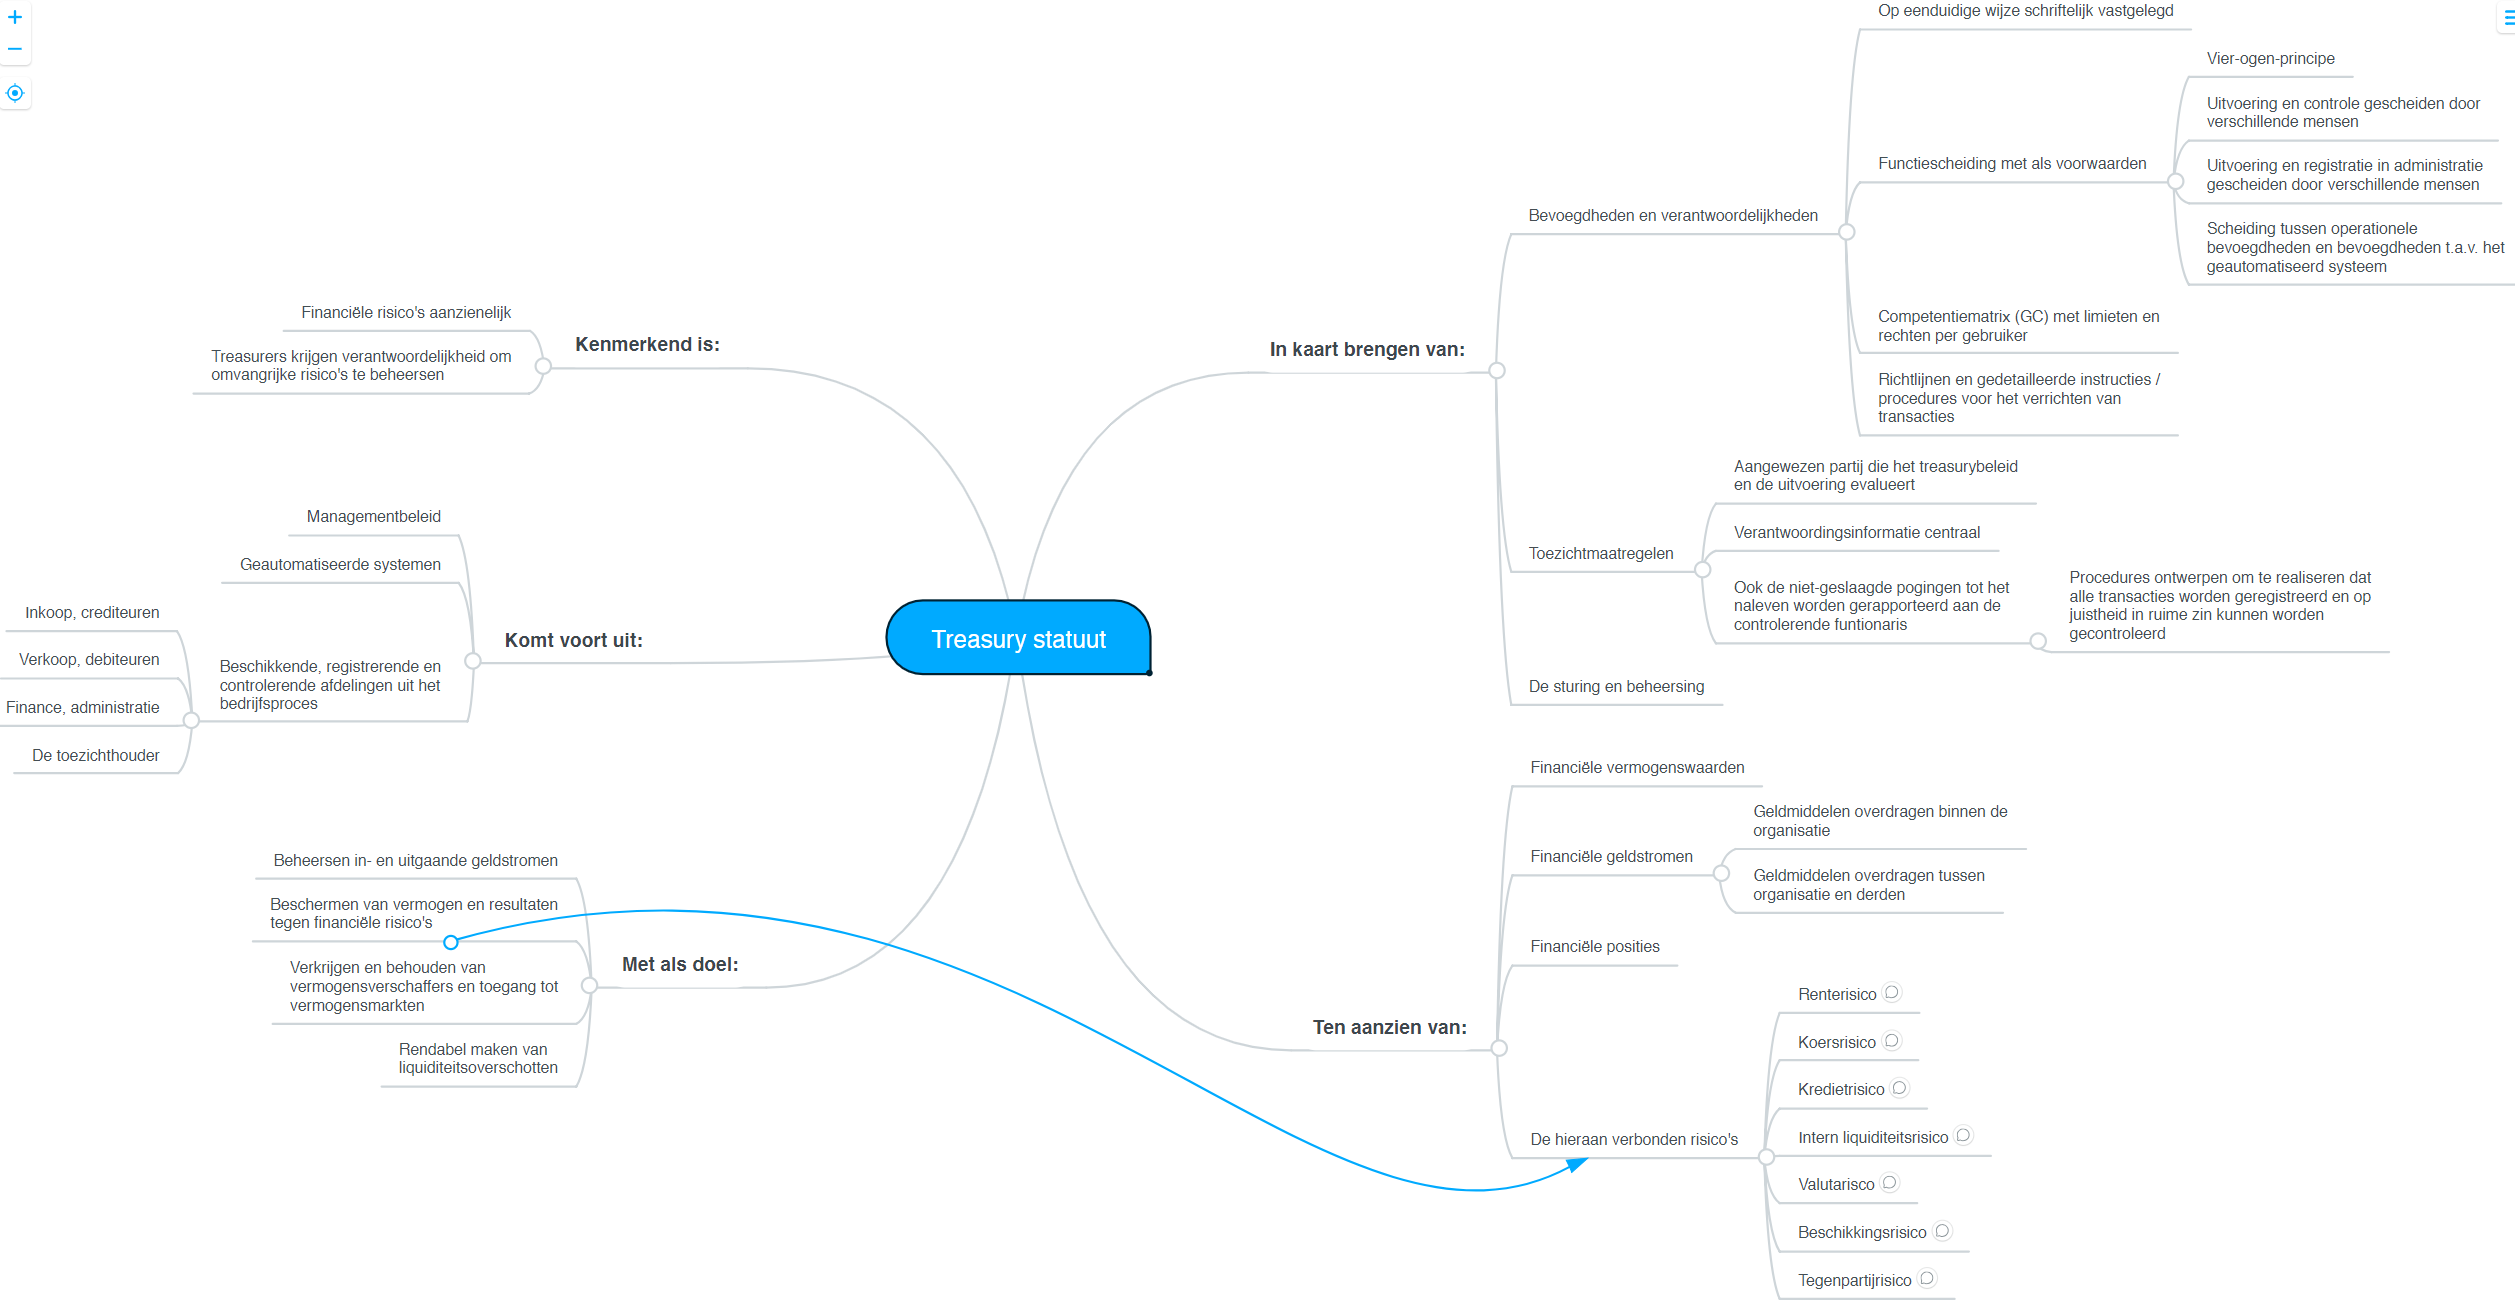
\includegraphics[angle=90,scale=0.245]{treasury}
    \label{fig:mmtreasury}
\end{figure}

\newpage

\subsection*{\hypertarget{bij:veldmodel}{Bijlage 2}: het causaal veldmodel \color{red}(schets)\color{black}}
\addcontentsline{toc}{section}{Bijlage 2: het causaal veldmodel}
\begin{figure}[ht]
    \centering
    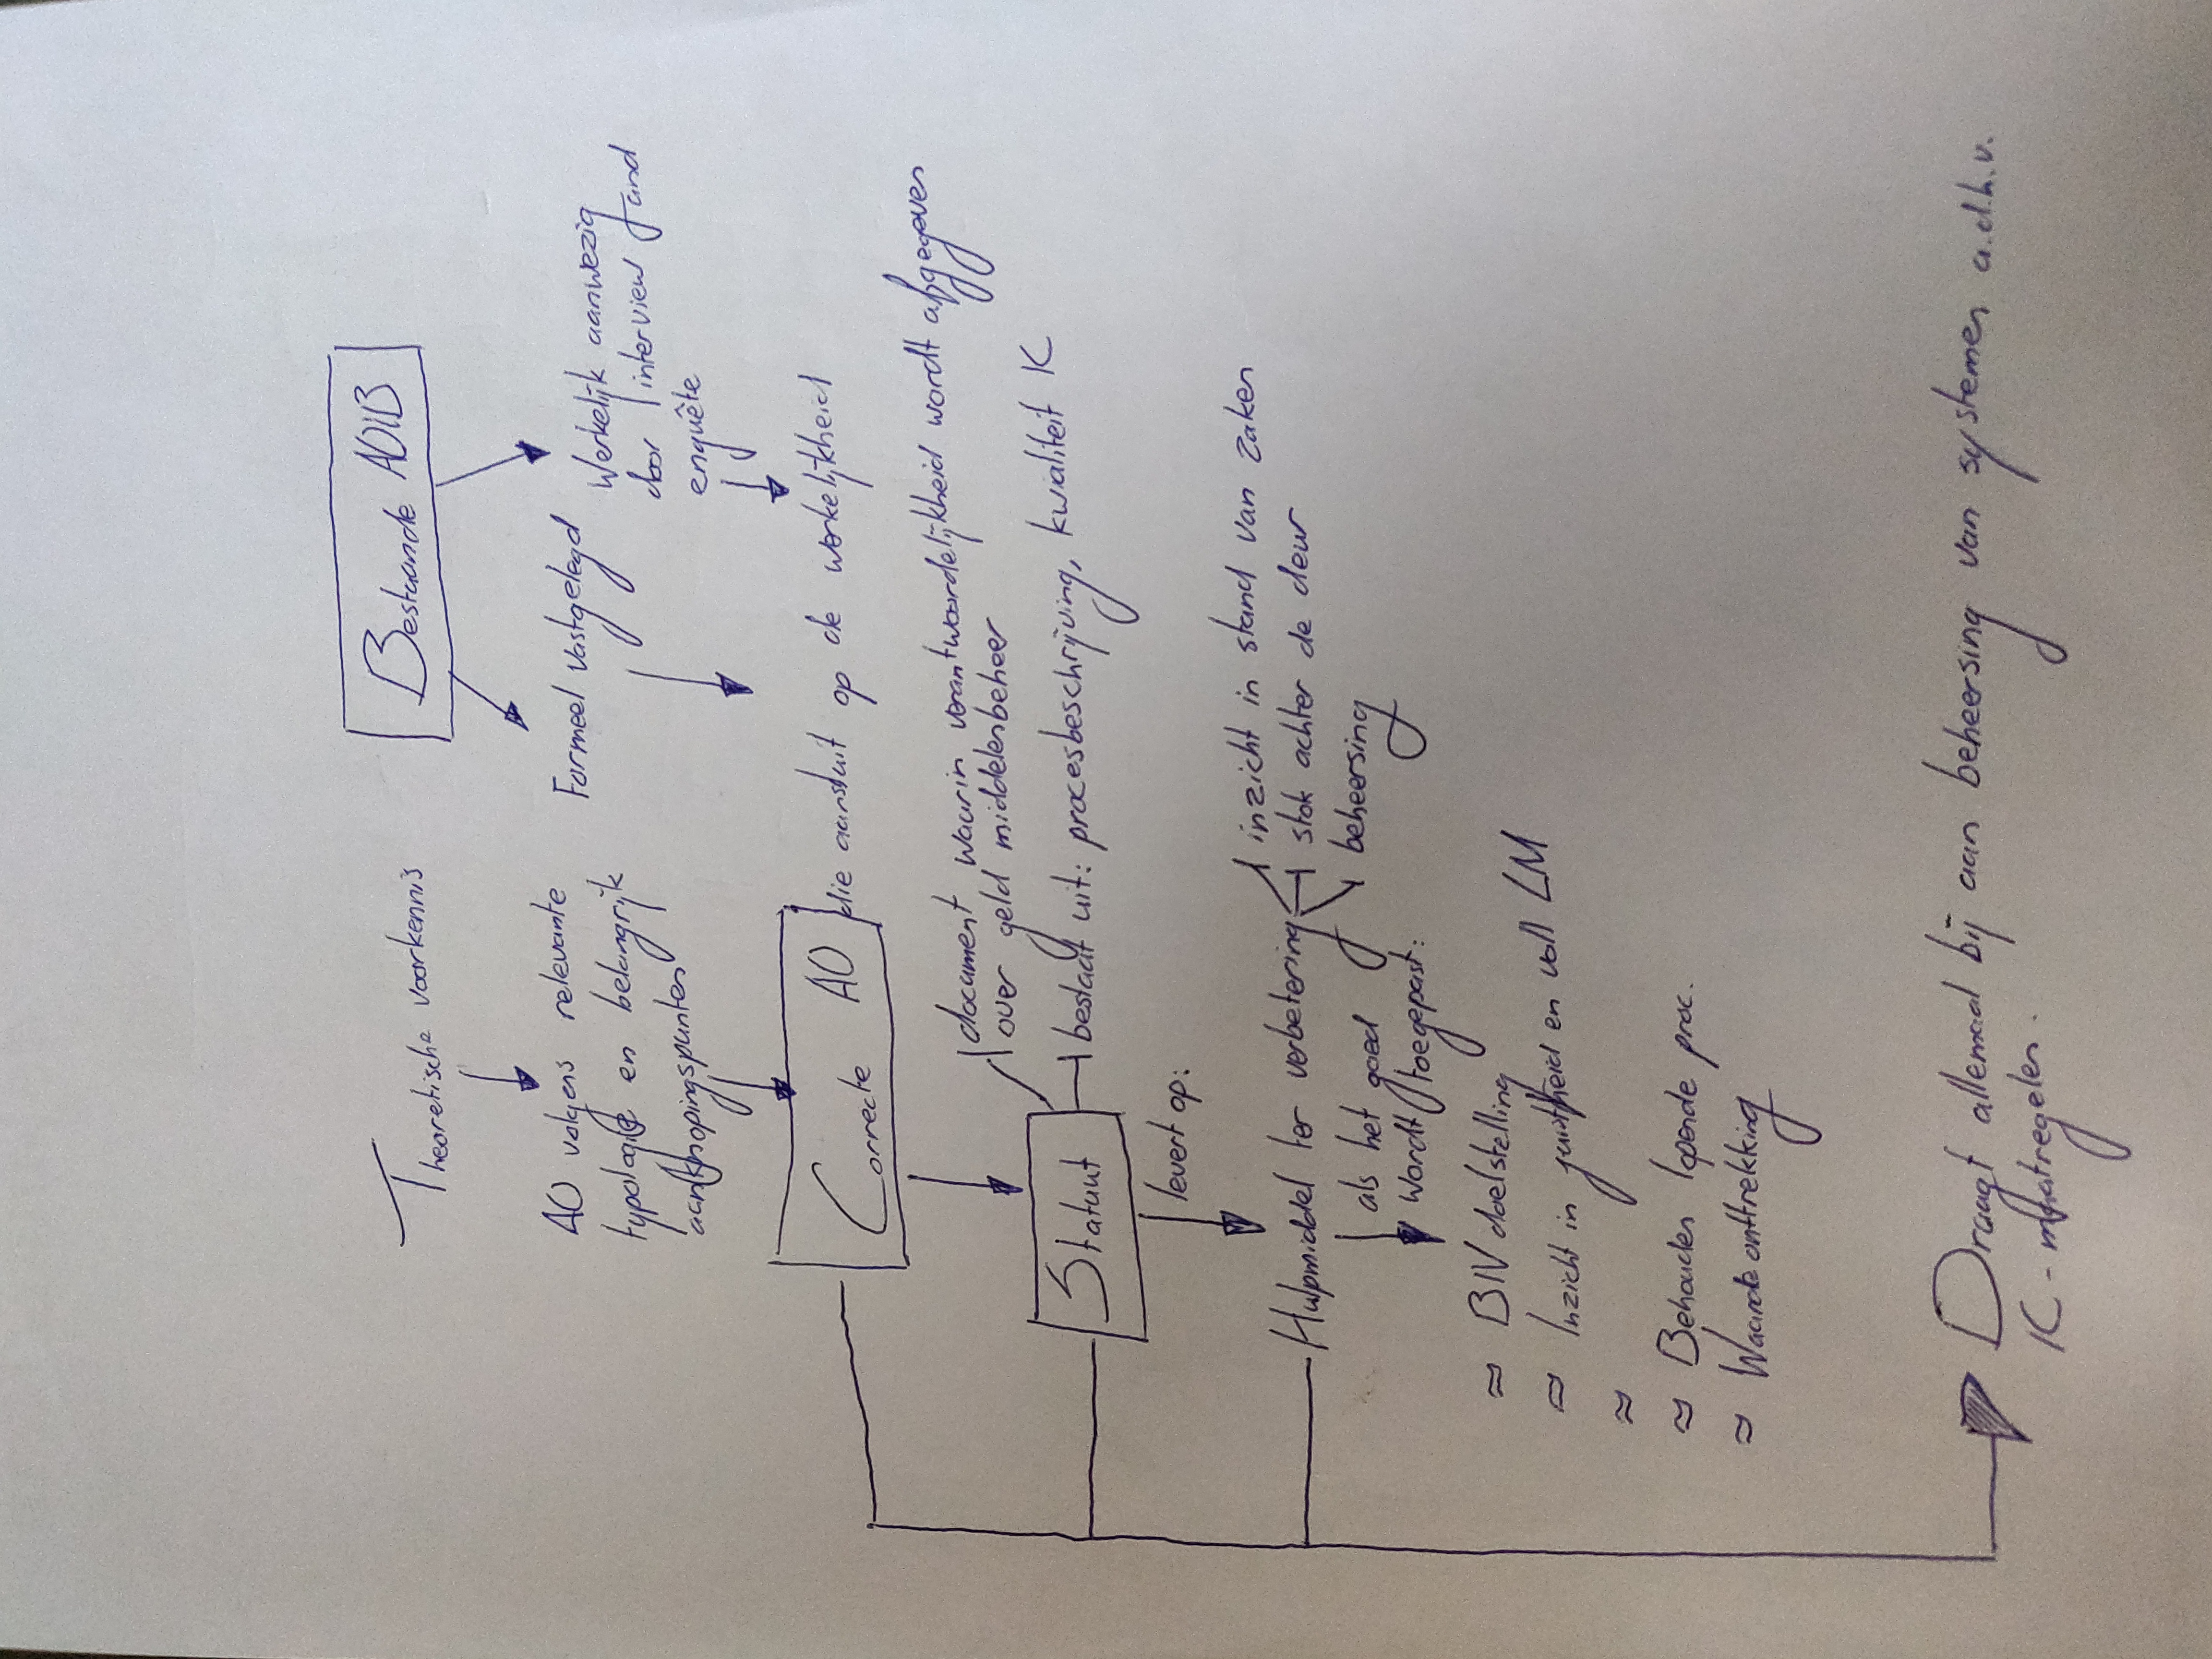
\includegraphics[angle=-90,scale=0.10]{veldmodel}
    \label{fig:veldmodel}
\end{figure}

\color{red}
\noindent
Mindmaps, voorwaardelijke interview- en enquêtevragen, treasury model?
\end{document}